\documentclass{article}

\usepackage[english]{babel}
\usepackage[letterpaper,top=2.5cm,bottom=2.5cm,left=2.5cm,right=2.5cm,marginparwidth=1.75cm]{geometry}
\usepackage{amsmath, graphicx, tikz, pgfplots, multirow, newlfont, gensymb, indentfirst, bm, setspace, fancyhdr, pdfpages, xurl}
\pagestyle{fancy}
\fancyhf{}
\rhead{Group 2 \\ 11/23/22}
\lhead{CE-321\\Structural Engineering}
\cfoot{\thepage}
\renewcommand{\headrulewidth}{1.5pt}
\setlength{\headheight}{22.6pt}
\usepackage[colorlinks=true, allcolors=black]{hyperref}
\setlength\parindent{24pt}
\pgfplotsset{scaled y ticks=false}
\pgfplotsset{scaled x ticks=false}
\pgfplotsset{width=12cm, compat=1.18}

\begin{document}
    \begin{titlepage}
    \begin{center}
    {{\Large{\textsc{The Cooper Union for the Advancement of Science and Art}}}} \rule[0.1cm]{15.8cm}{0.1mm}
    \rule[0.5cm]{15.8cm}{0.6mm}
    {\small{\bf DEPARTMENT OF CIVIL AND ENVIRONMENTAL ENGINEERING}}\\
    {\footnotesize{STRUCTURAL ENGINEERING LABORATORY}}
    \end{center}
    \vspace{15mm}
    \begin{center}
    {\large{\bf LAB 5\\}}
    \vspace{5mm}
    {\Large{\bf COMPRESSIVE TESTING OF\\}}
    \vspace{2mm}
    {\Large{\bf STANDARD CONCRETE CYLINDER}}
    \end{center}
    \vspace{35mm}
    \par
    \noindent
    \hfill
    \vspace{20mm}
    \begin{center}
    {\large{ {\bf Group 2} \\ { Jenna Manfredi\hspace{5mm}David Madrigal\hspace{5mm}Gila Rosenzweig\\Nicole Shamayev\hspace{5mm}Jake Sigman}}}
    \vspace{40mm}
    {\large {\bf \\CE-321 \\ 12/14/22 \\}}
    \vspace{15mm}
    {\normalsize{Professor Tzavelis \\ Avery Kugler \\ Lionel Gilliar-Schoenenberger \\ Crystal Woo}}
    \end{center}
\end{titlepage}
    \doublespacing
    \tableofcontents
    \newpage
    \addcontentsline{toc}{section}{List of Tables}
    \listoftables
    \addcontentsline{toc}{section}{List of Figures}
    \listoffigures
    \newpage
    \section{Objective}
    \indent Strain is the deformation of a material due to stress. The objective of this experiment is to measure the strain of a material with a strain gage as it is subjected to a force. To measure this deformation, it is necessary to connect a strain gage and terminal to a beam. The deformation is measured by connecting the gage terminal to a strain indicator via electrical wires. Knowing the strain of a material is vital in structural design since it shows how a material deforms. Any unanticipated deformation in a structure could be disastrous to its integrity. Therefore, strain is very important when choosing what material is best for a certain project.  The experiment is conducted in the Civil Engineering Structures Lab at the Cooper Union (room LL220). 
    \newpage
    \section{Procedure}
    \indent Installation of a strain gage is necessary to measure the strain at a point on a beam given increasing force. To install a strain gauge in the Cooper Union civil engineering lab, a detailed procedure was provided. The first step is to degrease the gaging area with Isopropyl Alcohol. This is followed by an abrading process with 400-grit silicon carbide paper, then dried by slowly wiping through with a gauze sponge. Using a pencil, an alignment mark is made on the specimen. Then using a cotton-tipped applicator and M-Prep Conditioner, all residue is removed until the tip is no longer discolored. The solution is closely monitored to make sure it doesn’t dry on the surface as this leaves a contaminating film. Then, apply a liberal amount of M-prep Neutralizer 5A and scrub with the cotton tipped applicator. Then the surface is dried with a gauze sponge. \\
    \indent Using tweezers, the gage is removed from the transparent envelope. A 6” piece of Micro-Measurements PCT gage instillation tape is placed over the gage and terminal. The tape is lifted at a 45-degree angle bringing the gage up with the tape. The gage/tape assembly is positioned so that the triangle alignment marks on the gage are over the layout lines on the specimen. The gage end of the tape is then lifted at a 45-degree angle until the gage and terminal are free of the specimen and surface. The loose end of the tape goes under, and the gage is pressed to the specimen surface, so it lies flat. M-Bond 200 catalyst is now applied to the bonding surface and terminal. The tucked edge of the tape is lifted, and the M-Bond 200 adhesive is applied to the fold formed by the junction of the tape and specimen surface. The tape is then rotated to a 30-degree angle so that the gage is bridged over the installation area. Then the gage/tape assembly is wiped down firmly followed by a thumb press directly on the gage and terminal area. This pressure is held for at least one minute. After the gage and terminal strip are bonded the tape is peeled off directly over itself to prevent lifting of the foil on the open-faced gage or other damage to the instillation. \\
    \indent After the strain gage is installed, the specimen is fixed on a beam and the gage is connected to electrical wires. These wires are connected to a strain indicator in the following fashion:
    \begin{center}
    \addcontentsline{lof}{figure}{Figure 1: Quarter Bridge Circuit Diagram}
    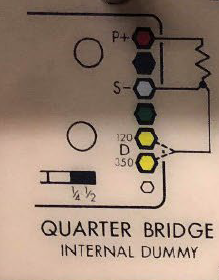
\includegraphics[scale=0.5]{fig1.png}
    \\Figure 1: Quarter Bridge Circuit Diagram
    \end{center}
    \indent\indent After the wires are connected, four equal weights are hung from the end of the beam and the readings on the strain indicator are recorded. \\
    \textbf{\underline{Handling Precautions:} } When the handling the M-Bond 200 please note that the immediate bonding of the eye, skin or mouth may result upon contact. This causes irritation. Avoid skin contact, prolonged or repeated breathing of vapors and use with adequate ventilation. \\
    \newpage
    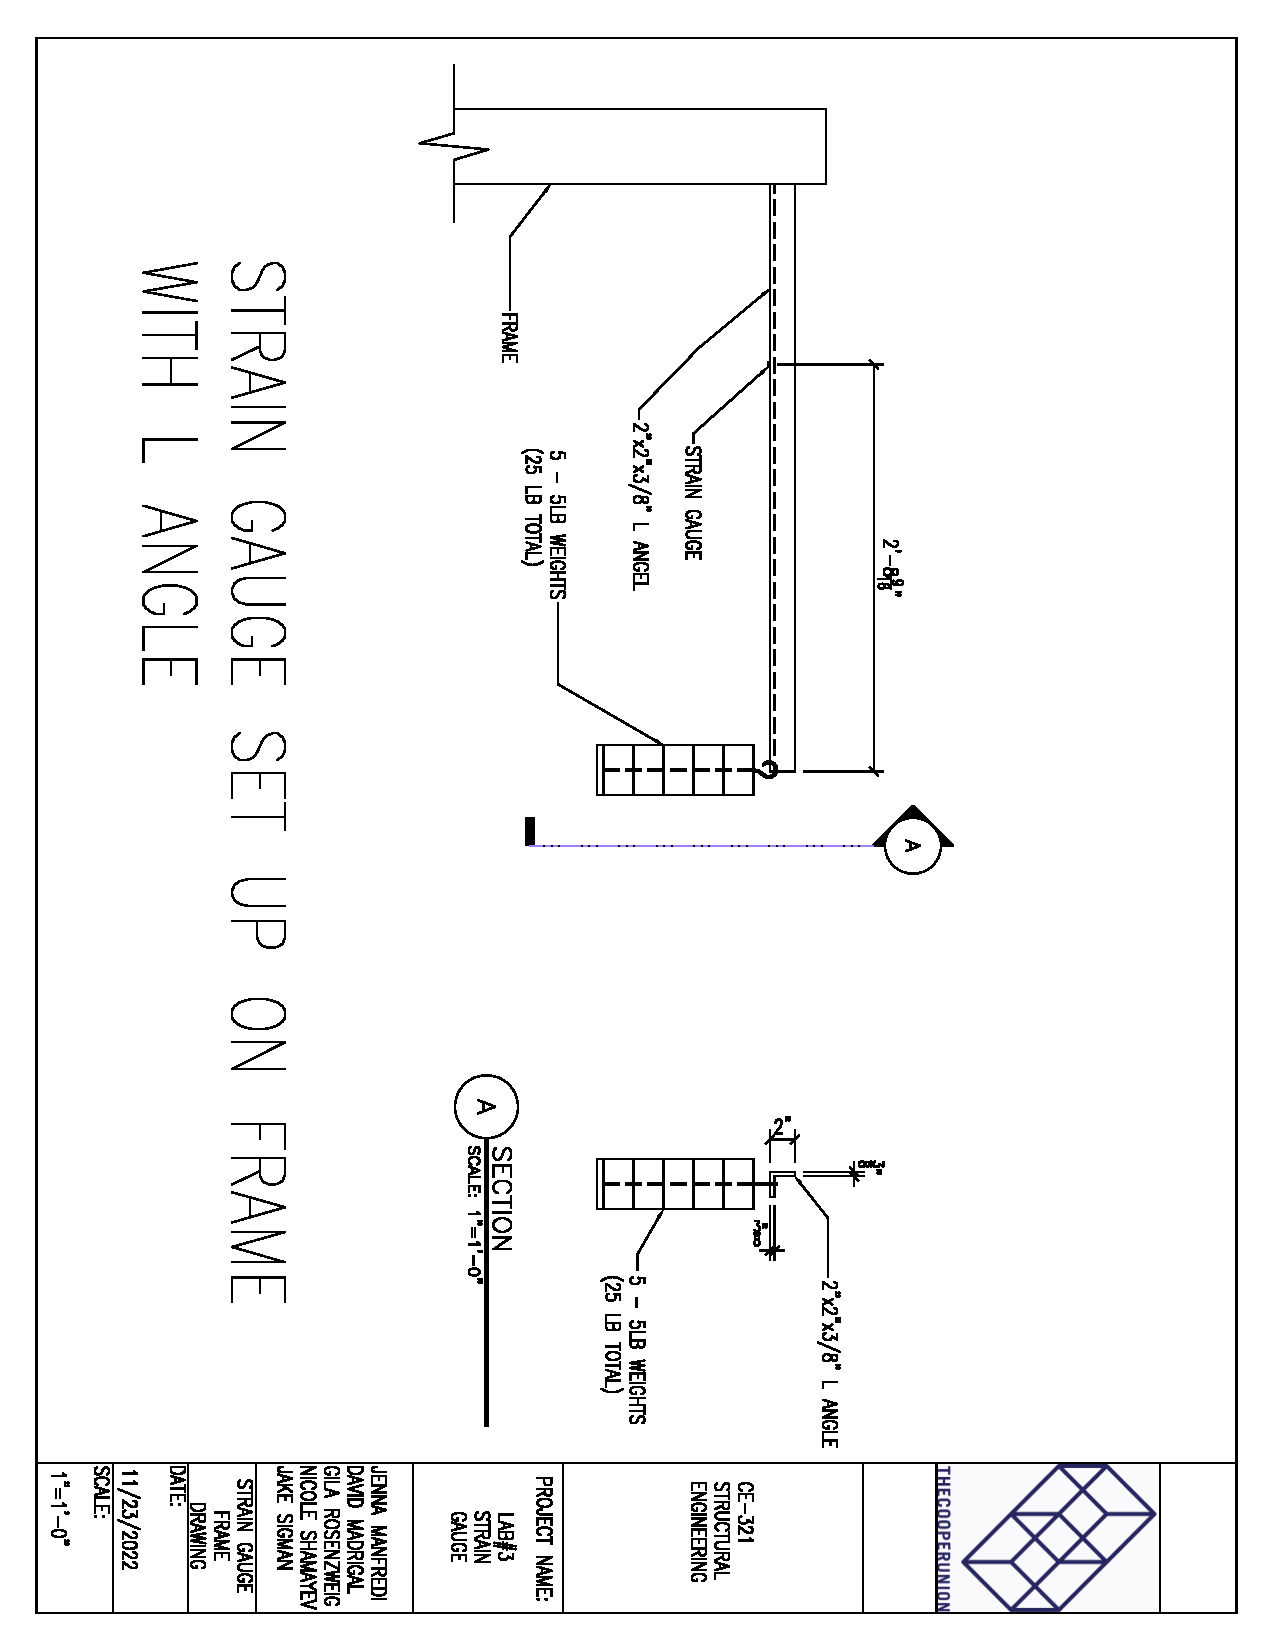
\includepdf[pages=-,pagecommand={\phantomsection\addcontentsline{toc}{subsection}{Equipment Drawing}\thispagestyle{empty}}]{dwg.pdf}
    \newpage
    \section{Theory}
    \noindent Consider a prismatic member undergoing a moment couple at both ends. A cubic element of the member will experience a uniaxial stress and strain; for a positive moment, the length of the top of the member will decrease due to compression and the length of the bottom will increase due to tension. Therefore, there exists a plane along the member where there is \emph{no change in length} due to a zero stress element. This is known as the \emph{neutral surface}; if considering a longitudinal section of the member it is defined as the \emph{neutral axis}.  \\
    Because the neutral axis preserves its length under flexure, the curvature that the member experiences is the reciprocal of the radius of the osculating circle $\rho$ and thus the original length of the neutral axis is defined by 
    \begin{equation*}
    L = \rho\times\theta 
    \end{equation*}
    where $\theta$ is the angle of the arc caused by bending. An arbitrary line $AB$ on the section with a positive vertical offset $y$ from the neutral axis will experience a deflection from flexure $\delta$, defined by the change in its original length $L$ to its new length after bending $L'$:
    \begin{equation*}
    \delta = L'-L 
    \end{equation*}
    The distance from the center of the circle to $AB$ is $\rho - y$; thus, the deflection that $AB$ undergoes is
    \begin{equation*}
        \delta = (\rho - y)(\theta) - \rho(\theta) = -y\,\theta 
    \end{equation*}
    Therefore, the longitudinal strain $\varepsilon_x$ is defined as the deflection over the original length:
    \begin{equation*}
        \varepsilon_x = \frac{\delta}{L} = \frac{-y\times\theta}{\rho\times\theta} = \frac{-y}{\rho}
    \end{equation*}
    The absolute maximum strain $\varepsilon_m$ occurs at the max distance from the neutral axis $c$:
    \[\varepsilon_m = \frac{c}{\rho}\]
    Thus, the relation between strain at a point and the maximum strain can be defined by combining with equation 4:
    \begin{equation*}
        \varepsilon_x = \frac{-y}{c}\,\varepsilon_m
    \end{equation*}
    If the stresses in the member are in the elastic range, Hooke's law applies for the bending stress $\sigma_x$:
    \[\sigma_x = E\times\varepsilon_x\]
    \[\sigma_x = \frac{-y}{c}\,\sigma_m\]
    The moment $M$ is defined by the magnitude of the force $\sigma_x dA$ multiplied by the distance from the neutral axis $y$ and assuming counterclockwise positive. The cubic stress element must be taken as an infinite sum to define the cross sectional area and therefore 
    \begin{equation*}
        M = \int\left[-y\times\sigma_x\right]dA
    \end{equation*}
    Substituting for maximum stress,
    \begin{equation*}
    M = \frac{\sigma_m}{c} \int y^2\,dA 
    \end{equation*}
    Because the moment of inertia $I$ is defined to the second moment of area, the equation for maxmimum bending stress as a function of moment can be written as:
    \begin{equation*}
        \sigma_m = \frac{M\times c}{I}
    \end{equation*}
    Lastly, back substituting for bending stress at an arbitrary line $\sigma_x$:
    \begin{equation*}
        \sigma_x = \frac{-M\times y}{I}
    \end{equation*}
    Equations 8 and 9 are defined as the \emph{flexure formula} for maximum bending stress and bending stress at an arbitrary point respectively.
    \\\\
    For this laboratory experiment, the bending stress of a cantilevered beam will be determined theoretically from the flexure formula and empirically using a \emph{strain gauge}. A strain gauge converts a force into a change in electrical resistance; the strain gauge is connected to an electrical circuit that measures changes in resistance; a quarter-bridge electrical circuit defines the resistance of the strain gauge as a function of two other known resistances and a third resistance given by an empirically defined gauge factor. Thus, the strain in the member can be experimentally determined by installing the strain gauge on the surface of the beam and forming the quarter-bridge circuit. 

    \newpage
    \section{Sample Calculations}
    \singlespacing
    \subsection{Beam Neutral Axis}
    \[y=\frac{b\,t-t^2+d^2}{2\,(b-t+d)}\]
    \[y=\frac{2\times0.375-0.375^2+2^2}{2\,(2-0.375+2)}=\boxed{0.636\text{ in}}\]
    \subsection{Moment of Inertia}
    \[I=\frac{1}{3}\,t\left[b\left(t^2-3\,t\,y+3\,y^2\right)+d\left(d^2-3\,d\,y+3\,y^2\right)+t\left(-t^2+3\,t\,y-3\,y^2\right)\right]\]
    \begin{multline*}
        I=\frac{1}{3}\,t\,[2\left(0.375^2-3\times0.375\times0.636+3\times0.636^2\right)+2\left(2^2-3\times2\times0.636+3\times0.636^2\right)\\+0.375\left(-0.375^2+3\times0.375\times0.636-3\times0.636^2\right)]=\boxed{0.492\text{ in}^4}
    \end{multline*}
    
    \subsection{Applied Moment}
    \[M=P\times L\]
    \[M=1\text{ lb}\times 32.56\text{ in}=\boxed{32.56\text{ lb}\cdot\text{in}}\]
    \subsection{Theoretical Stress}
    \[\sigma_\text{Th}=\frac{M\times y}{I}\]
    \[\sigma_\text{Th}=\frac{32.56\text{ lb}\cdot\text{in}\times 0.636\text{ in}}{0.492\text{ in}^4}=\boxed{42.05\text{ psi}}\]
    \subsection{Theoretical Strain}
    \[\varepsilon_\text{Th}=\frac{\sigma_\text{Th}}{E}\]
    \[\varepsilon_\text{Th}=\frac{42.05\text{ psi}}{10\times10^6\text{ psi}}=\boxed{7.5\times10^{-6}}\]
    \subsection{Experimental Stress}
    \[\sigma_\text{Exp}=\varepsilon\times E\times r_\text{Gauge}\]
    \[\sigma_\text{Exp}=\left(40\times10^{-6}\right)\times \left(10\times10^6\text{ psi}\right)\times\left(\frac{1.2}{2.14}\right)=\boxed{224.30 \text{ psi}}\]
    \newpage
    \section{Results}
    \doublespacing
    \begin{center}
    \addcontentsline{lot}{table}{Table 1: Experimental and Theoretical Results}
    {\large{\bf Table 1: Experimental and Theoretical Results\\}}
    \vspace{3mm}
    \begin{tabular}{|c c c c c|}
        \hline
        \textbf{P (lb)} & \(\bm{\mu\varepsilon}_\textbf{Exp}\) & \(\bm{\mu\varepsilon}_\textbf{Th}\) & \(\bm{\sigma}_\textbf{Exp}\)\textbf{ (psi)} & \(\bm{\sigma}_\textbf{th}\)\textbf{ (psi)}\\ \hline
        1&  0&      7.50&       0&          42.05\\
        5&  40&     37.50&      224.30&     210.27\\
        10& 80&     75.00&      448.6&      420.55\\
        15& 119&    112.50&     667.29&     630.82\\
        20& 158&    150.00&     885.98&     841.10\\
        25& 197&    187.49&    1104.67&    1051.37\\\hline
    \end{tabular}
    \vspace{5 mm}
    \addcontentsline{lot}{table}{Table 2: Error Percentages}
    {\large{\bf \\Table 2: Error Percentages\\}}
    \vspace{3mm}
    \begin{tabular}{|c c|}
        \hline
        \(\bm{\sigma}\) & \(\bm{\varepsilon}\) \\\hline
        100\% & 100\% \\
        6.67\% & 6.67\% \\
        6.67\% & 6.67\% \\
        5.78\% & 5.78\% \\
        5.34\% & 5.34\% \\
        5.07\% & 5.07\% \\
        \hline
    \end{tabular}
    \end{center}
    \newpage
    \newpage
    \begin{center}
    \doublespacing
        \begin{tikzpicture}[baseline=(current bounding box.center)]
            \addcontentsline{lof}{figure}{Figure 2: Stress vs. Strain Curve}
            \begin{axis}[
                title={\textbf{Figure 2: Stress vs. Strain Curve}},
                xlabel={\(\mu\varepsilon\)},
                ylabel={\(\sigma\) (psi)},
                ymin=0, ymax=1500,
                xmin=0, xmax=200,
                ytick={0,500,1000,1500},
                xtick={0,50,100,150,200},
                ymajorgrids=true,
                grid style=dashed,
                cells={anchor=west},
                width=0.9\textwidth,
                height=1.3\textwidth,
                legend cell align={left}
            ]
            
            \addplot[only marks, red] table [x=strain, y=stress] {fig1.csv};
            \addplot[only marks, blue] table [x=th_strain, y=th_stress] {fig1.csv};
            \addplot[dashed, red, domain=0:200] {5.6075*x};
            \addplot[dotted, blue, domain=0:200] {5.6075*x};
            \addlegendentry{Experimental}
            \addlegendentry{Theoretical}
            
            
            \end{axis}
        \end{tikzpicture}
    \end{center}
    \newpage
    \section{Conclusion}
    \indent In comparing experimental to theoretical data, it is important to note that while theoretical data has non-zero values for stress and strain with the application of a 1 pound load, experimental data shows values of zero for each; this is due to the fact that the gauge was zeroed after the application of 1 pound of loading, for the purposes of achieving more accurate relative measurements. If the experiment proceeds as expected, the same linear relationship between stress and strain should be seen, despite the initial differences. \\
    \indent Plotting the stress v. (micro)strain curve produces a linear relationship, demonstrating that the deflection is elastic. When compared to a plot of the theoretical stress and strain, the same linear relationship is produced, indicating that the beam is behaving as is materially expected. The differences in values between theoretical and experimental data are relatively small (carrying percent errors of less than 7\%, with the exception of stress and strain at one pound of loading, at 100\% error due to zeroing) and can be attributed to a variety of factors. (Of note, strain in this experiment is recorded as microstrains, and as such, differences are small, but can have significant impact as they appear in the denominator of the ratio.)  Firstly, differences are introduced between theory and experiment by the zeroing of the gauge with the application of a one-pound load. Further error and differences can be introduced by the testing environment: magnetostrictive effects, hydrostatic pressure, and high humidity can all potentially introduce error. Instrumental error is possible if the wiring used in the quarter-bridge is not properly insulated and is therefore subject to external factors which can change resistance in the circuit. Procedural error is possibly introduced if readings are taken before vibrations settle and the gauge is thus not stabilized at a constant value; another potential error is the possibility that the weights added to the loading are not accurately described and may be heavier or lighter than marked. \\
    \indent Despite the opportunity for several sources of error to have affected the experiment, the values still produce the same linear relationship as did the theoretical values; given that, it is reasonable to assume that the beam has the recorded modulus of elasticity and other material properties. It is also fair to say that the gauge is working as expected, subject to normal variation. To improve this experiment for future iterations, it would make sense to zero the gauge at no loading, rather than at one pound, if it is feasible; this would give the experimental and theoretical data the same starting values, and allow comparisons of differences to be more accurate. It would also be wise to reduce external vibrations which can affect results; this includes vibration of the frame and floor, as well as waiting a bit more time after an increase in load to ensure readings can stabilize and no one is touching or shaking the gauge setup. \\
    \indent Strain gauge technology is often used in field conditions. Potential such uses are testing vehicles, ship hulls, dams, and oil drilling platforms. Gauges can be installed on structural components in a bridge or building to monitor stress and compare it with analytical models and calculations. Laboratory testing is different than field testing because the field environment introduced complex shapes, geometries, access, and a host of other variables more subject to variation than in a lab. Some field conditions require custom gauge manufacturing to properly capture the subtle changes in pressure and/or stress. \\
    \indent Particular civil engineering applications of strain gauge use include monitoring bridge cables. In bridge applications, strain gauges allow for real-time monitoring that enable inspections to be more thorough and reduce possibilities for an inspector to miss signs of structural damage. Strain gauges have also been used in bridge rebuilds, to monitor bridge response to overload and speeding vehicles, monitor displacements, and sense wind speed and its resulting strain on cables. \\
    \indent Strain gauges can also be installed for rail monitoring. One such examples Is places where a rail line is in place atop a mine, where subsidence-related ground shear may require the installation of expansion switches, the activation of which may be triggered by threshold values off the strain gauge. A more typical rail application is in measuring axial tension and compression on rails without impacting the rails themselves, for the purpose of triggering a warning to maintenance personnel when subsidence occurs. \\
    \indent The intent behind using a strain gauge for flexural testing of a beam is to provide an understanding of the function and utility of a strain gauge and how it may be used in field applications. Field conditions can call for flexural testing, as well as other stress responses of structural members in buildings and bridges. The use of a strain gauge can be helpful in determining if a member is behaving as expected, or is displaying signs of fatigue or failure. 
    \newpage
    \section{References}
    \begin{description}
        \item Ferdinand B. \emph{et. al.} (2015). \emph{Mechanics of Materials}, 7th Ed., McGraw Hill, New York.
        \item Wilson, E. \emph{Strain-Gage Instrumentation}.
        \item Nachazel, T. (2020). What is a Strain Gauge and How Does it Work?, \url{https://www.michsci.com/what-is-a-strain-gauge/} (accessed 20 November 2022).
        \item Sensing Systems (2018). Strain Gauge Technology in Field Testing, \url{https://www.sensing-systems.com/blog/strain-gauge-technology-in-field-testing#:~:text=Strain%20gauges%20are%20used%20to,rotational%20speed%20on%20a%20shaft} (accessed 20 November 2022).
        
    \end{description}
    \newpage
    \section{Appendix}
    \begin{center}
    \noindent Beam Length, \(L\) (ft): 2.71\\
    Vertical Leg Length, \(d\) (in):  2\\
    Horizontal Leg Length, \(b\) (in): 2\\
    Thickness, \(t\): 0.38\\
    Beam Neutral Axis, \(y\): 0.64\\
    Beam Cross-Sectional Area, \(A\) (\(\text{in}^2\)): 1.36\\
    Moment of Inertia, \(I\) (\(\text{in}^4\)): 0.49\\
    Modulus of Elasticity, E (psi): 10000000\\
    \end{center}
    \begin{center}
        \begin{tabular}{|c | c | c c | c c|}
            \hline
            \textbf{P (lb)} & \textbf{M (lb\(\cdot\)in)} & \(\bm{\sigma}_\textbf{Th}\)\textbf{ (psi)} & \(\bm{\mu\varepsilon}_\textbf{Th}\) &  \(\bm{\sigma}_\textbf{Exp}\)\textbf{ (psi)} & \(\bm{\mu\varepsilon}_\textbf{Exp}\)\\ \hline
            1&  32.56&      0&       7.50&               42.05&    0\\\hline
            5&  162.81&     224.30&        37.50&      210.27&   40\\\hline
            10& 325.63&     448.60&      75.00&      420.55&   80\\\hline
            15& 488.44&     667.29&        112.50&     630.82&   119\\\hline
            20& 651.25&     885.98&      150.00&     841.10&   158\\\hline
            25& 814.06&     1104.67&     187.49&     1051.37&  197\\\hline
        \end{tabular}
    \end{center}
\end{document}